\documentclass[11pt]{sdm}
\usepackage{graphicx}
\usepackage{subcaption}
\usepackage{textcomp}
\usepackage[francais]{babel}

%numeroter les pages
\pagestyle{plain}

\title{Deep Learning and Time Series}
\author{Arthur \textsc{Le Guennec}}
\supervisorOne{Romain \textsc{Tavenard} of your first supervisor}
\supervisorTwo{Simon \textsc{Malinowski} of your second supervisor}
\team{OBELIX}
%One of:
% ens-Rennes  esir    insa-rennes logoENIB  rennes1  UBO
% enssat header logo_ENIB   logoUbs   tel-br supelec

\school{rennes1}


% the domain should be one or two of:
% Technology for Human Learning 
% Artificial Intelligence 
% Computer Arithmetic
% Hardware Architecture
% Automatic Control Engineering
% Bioinformatics 
% Biotechnology
% Computational Complexity 
% Computational Engineering, Finance, and Science
% Computational Geometry 
% Computation and Language 
% Cryptography and Security 
% Computer Vision and Pattern Recognition
% Computers and Society 
% Databases 
% Distributed, Parallel, and Cluster Computing 
% Digital Libraries
% Discrete Mathematics 
% Data Structures and Algorithms 
% Embedded Systems 
% Emerging Technologies 
% Formal Languages and Automata Theory 
% General Literature 
% Graphics 
% Computer Science and Game Theory 
% Human-Computer Interaction 
% Computer Aided Engineering 
% Medical Imaging 
% Information Retrieval 
% Information Theory 
% Ubiquitous Computing 
% Machine Learning
% Logic in Computer Science 
% Multiagent Systems 
% Mobile Computing
% Multimedia
% Modeling and Simulation 
% Mathematical Software 
% Numerical Analysis 
% Neural and Evolutionary Computing 
% Networking and Internet Architecture 
% Operating Systems 
% Performance 
% Programming Languages 
% Robotics 
% Operations Research
% Symbolic Computation 
% Sound
% Software Engineering 
% Social and Information Networks 
% Systems and Control 
% Image Processing 
% Signal and Image Processing 
% Document and Text Processing
% Web
\domain{Domain:  (examples) Data Structures and Algorithms - Logic in Computer Science}

%write your abstract here
\abstract{write your abstract here}



\begin{document}
\maketitle

%*****************************************************************%

\section{Introduction}

Il y a beaucoup d\textquotesingle articles sur la classification des s\'eries temporelles, et est présente dans beaucoup de domaine comme la m\'edecine, la biologie, la reconnaissance audio, ... Il existe beaucoup de m\'ethodes diff\'erentes pour y parvenir. Par exemple, le document \cite{bailly2015bag} utilise les bag-of-words, une technique bas\'ee sur la description des documents par des mots. \cite{zheng2014time} utilise plut\^ot les r\'eseaux de neurones convolutionnels.
Dans ce document, nous allons utiliser les r\'eseaux de neurones profonds. Dans ce type de mod\`ele d\textquotesingle apprentissage, les r\'eseaux convolutionnels (ou Convolutional Neural Networks) ont de tr\`es bons r\'esultats dans le domaine de la classification d\textquotesingle image (\cite{chatfield2014return}).
Comme dans le domaine des s\'eries temporelles les nombres de donn\'ees annot\'ees est faible, on allons explorer des m\'ethodes permettant de diminuer les cons\'equequences de ce manque de donn\'ees. \\
Ce papier est organis\'e de la mani\`ere suivante. La section 2 concerne l'\'etat de l'art dans ce domaine, la section 3 introduit les outils qui vont nous servir pour la classification, et la section 4 s'interessera aux probl\`emes qui nous concernent.

% Ce sujet de stage propose de s’int\'eresser \`a la classification de s\'eries temporelles en utilisant des mod\`eles d’apprentissage tr\`es puissants : les r\'eseaux de neurones profonds (Deep Neural Networks). Dans cette famille de m\'ethodes, les r\'eseaux convolutionnels (Convolutional Neural Networks, CNN) montrent actuellement l’\'etendue de leurs capacit\'es dans le domaine de la vision par ordinateur (voir par exemple [1]). Les tr\`es bonnes performances des CNN s’expliquent par leur capacit\'e \`a tirer profit des grands volumes de donn\'ees disponibles pour apprendre des descriptions et des classifieurs complexes. Dans le domaine de la classification de s\'eries temporelles, les volumes de donn\'ees annot\'ees sont souvent bien plus faibles [2]. L’objet de ce stage est d’\'evaluer la pertinence de l’utilisation des CNN dans ce cadre et de proposer des moyens d’att\'enuer l’impact attendu du faible volume de donn\'ees annot\'ees [3]. L’\'etudiant(e) retenu(e) devra faire preuve d’organisation et de s\'erieux pour mener \`a bien la campagne exp\'erimentale intensive impliqu\'ee par ce sujet. Pour ce faire, il/elle utilisera le framework Caffe [4].
 

\section{State of the art}
	La classification de s\'erie temporelle est un sujet qui est \'etudi\'e depuis maintenant plusieurs ann\'ees, donc diff\'erentes techniques existent et de nombreux articles sur le sujet. Dans cette partie nous allons voir quelques unes de ces diff\'erentes techniques.
	\subsection{Bag-of-Words}	
		Le Bag-of-Words (BoW) est un mod\`ele de description de document avec des descripteurs (des “mots”). Il fonctionne en attribuant des mots aux documents, chaques mots ayant un probabilit\'e par document (voir figure~\ref{fig:Bow}). \cite{bailly2015bag} traite justement le sujet de la classification des s\'eries temporelles avec les Bag-of-Words.

		\begin{figure}[!ht]
			\centering
			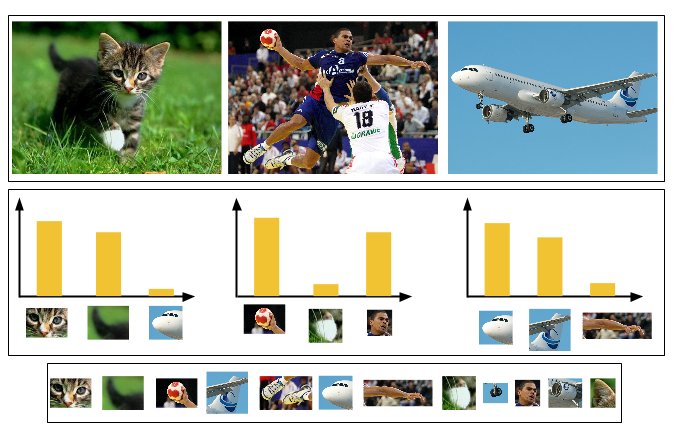
\includegraphics[scale=0.6,natwidth=680,natheight=440]{figures/bagOfWords.png}
			\caption{Le bag-of-words est en bas de la figure, il est compos\'e de diff\'erents mots, ici des images, qui sont reconnus sur les documents (en haut), qui sont ici des images. Par exemple, pour la premi\`ere image, on a une forte correspondance avec le premier et deuxi\`eme mot, alors que l’on a une faible correspondance avec la derni\`ere image.}
			\label{fig:BoW}
		\end{figure}

	\subsection{Support Machine Vector}
		Les SVM (Support Vector Machine ou Machine \`a Vecteur de Support en fran\c cais) sont des techniques d\textquotesingle apprentissage supervis\'e. 



\section{Neurals Networks and Time Series}
	\subsection{Neural Network}
		Les r\'eseaux de neurones sont un syst\`eme inspir\'e du mod\`ele biologique du cerveau. Un r\'eseau de neurone est compos\'e de plusieurs neurones (voir figure~\ref{fig:neuralNetwork}) qui ont chacun une fonction d’activation (voir figure~\ref{fig:neural}) et qui sont reli\'es \`a d\textquotesingle autres neurones par des poids.

		\bigbreak

		\begin{figure}[!ht]
			\centering
			\begin{subfigure}{0.45\textwidth}
				\centering	
				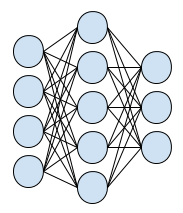
\includegraphics[scale=0.7,natwidth=183,natheight=213]{figures/neuralNetworkLayers.png}
				\caption{R\'eseau de neurones \`a couches}
				\label{fig:nnl}
			\end{subfigure}
			\hspace*{\fill}
			\begin{subfigure}{0.45\textwidth}	
				\centering
				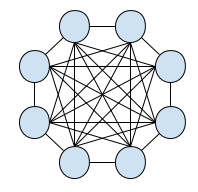
\includegraphics[scale=0.7,natwidth=198,natheight=192]{figures/neuralNetworkCompleteConnexion.png}
				\caption{R\'eseau de neurones \`a connexion compl\`ete}
				\label{fig:nnc}
			\end{subfigure}
			\caption{Il existe diff\'erents types de r\'eseaux de neurones. Par exemple, la figure 1.a est un r\'eseau avec une architecture \`a couche, alors que le r\'eseau de la figure 2.b \`a une architecture \`a connexion compl\`ete. Dans le domaine de la classificatin, l'architecture \`a couche est souvent utilis\'e.}
			\label{fig:neuralNetwork}
		\end{figure}

		\bigbreak

		\begin{figure}[!ht]
			\centering
			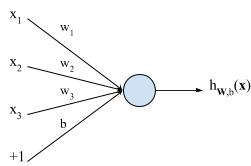
\includegraphics[natwidth=131,natheight=52]{figures/neural.png}
			\caption{La fonction d\textquotesingle activation est la fonction qui va d\'eterminer le comportement du neurone. Par exemple, si la fonction d\textquotesingle activation est un threshold, la sortie sera soit 1, soit 0. Si c’est une sigmoide (le plus souvent utlis\'e), la sortie sera y = 1 / (1 + exp(-x)) avec y la sortie et x l\textquotesingle entr\'ee.}
			\label{fig:neural}
		\end{figure}
	
		\bigbreak
		\bigbreak

		L\textquotesingle un des avantages d\textquotesingle un r\'eseau de neurones est qu\textquotesingle il s\textquotesingle agit d\textquotesingle un syst\`eme qui apprend par entra\^inement. Il y a donc deux \'etapes pour un r\'eseau de neurone, d’abord l\textquotesingle entra\^inement, puis la v\'erification. Un autre avantage est qu\textquotesingle il donne souvent de bons r\'esultats, de nombreux papiers sur le sujet obtiennent souvent des taux d’erreurs tr\`es faibles (mettre les r\'ef\'erences ici).
		Comme vu pr\'ec\'edemment, il y a deux \'etapes essentielles pour le fonctionnement d’un r\'eseau de neurones : l\textquotesingle entra\^inement et le test. L\textquotesingle entra\^inement est l\`a pour trouver les poids corrects entre les neurones, et le test pour v\'erifier que ces poids sont corrects. Dans les deux cas, le r\'eseau a besoin d\textquotesingle une base de donn\'ee sur laquel s\textquotesingle entra\^iner et tester. Cette base de donn\'ee sera alors s\'epar\'ee en deux parties, l\textquotesingle une pour l\textquotesingle entra\^inement, une autre pour le test.
		L\textquotesingle efficacit\'e d\textquotesingle un r\'eseau de neurones d\'epend de son architecture. Selon le nombre de couche et le nombre de neurones par couche, le r\'eseau peut \^etre plus ou moins performants (\cite{chatfield2014return}\cite{srivastava2014dropout}). La taille de la base de donn\'ee utilis\'e influence aussi les r\'esultats, Par exemple, [J\textquotesingle ai oubli\'e la r\'ef\'erence] montre bien que les performances d\'ependent bien de la taille des donn\'ees utilis\'ees. \begin{itshape} Rajouter que les m\'ethodes influencent aussi sur le r\'esultats. \end{itshape}


	\subsection{CNN}
		Les CNN (Convolutional Neural Network, ou r\'eseaux convolutionnels) sont un structure particuli\`ere des r\'eseaux de neurones car les neurones d\textquotesingle une couche \`a une autre ne sont pas tous reli\'es entre eux comme dans un r\'eseau de neurone \`a couche classique (voir figure~\ref{fig:nnc}). Les connections entre neurones se font localement, ce qui fait des entr\'ees d\textquotesingle une couche cach\'ee un sous-ensemble de motif de la couche pr\'ec\'edente. La figure~\ref{fig:cnn} illustre bien l\textquotesingle architecture d'un CNN.

		\begin{figure}[!ht]
			\centering
			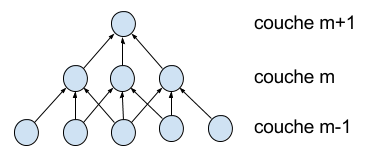
\includegraphics[natwidth=375,natheight=152]{architectureCNN.png}
			\caption{Ici, imaginons que la couche m-1 est une r\'etine o\`u chaque neurone correspond \`a un pixel d\textquotesingle une image. Dans la couche m, on s\textquotesingle aper\c coit que chaque neurone a 3 entr\'ees qui correspondent chacune \`a un pixel. Chaque neurone de la couche m est donc un sous-ensemble de l\textquotesingle image de 3 pixels. De la m\^eme fa\c con, chaque neurone de la couche m+1 est donc un sous-ensemble de l\textquotesingle image de 5 pixels.}
			\label{fig:cnn}
		\end{figure}


	\subsection{Time Series}
		Les s\'eries temporelles sont des donn\'ees qui d\'ependent du temps. Par exemple, la taille d\textquotesingle une personne par rapport \`a son âge peut \^etre vu comme une s\'erie temporelle. Le document [1] nous donne les d\'efinitions qui nous seront utile par la suite.
		Il existe de nombreux domaines o\`u les s\'eries temporelles interviennent. Elles peuvent, par exemple, servir dans la biologie, la m\'edecine, la finance, ...



\section{Data-augmentation for Time Series}
	\subsection{Pourquoi chercher \`a augmenter la base de donn\'es ?}
		On a besoin de palier le manque de donn\'ee car les structures CNN ont besoin de beaucoup de donn\'ees pour pouvoir \^etre entra\^in\'es efficacement. Les structures tels que MC-DCNN (voir \cite{zheng2014time}) peuvent \^etre utilis\'e.
		De plus il y a peu, compar\'es aux images, de donn\'ees sur les s\'eries temporelles. On aura donc besoin d\textquotesingle augmenter ces donn\'ees de diff\'erentes fa\c cons.
		Par analogie aux images, on regardera comment transformer une s\'erie temporelle. Dans les donn\'ees pour les images, on applique certaines transformations, tel que la translation, l\textquotesingle inversion, le changement de couleur, de contraste, de luminosit\'e, ... (voir figure~\ref{fig:dataAugmentationChat}). Ces transformations ne sont pas applicables directment aux s\'eries temporelles.

	\subsection{Comment y parvenir ?}
		Pour les images, plusieurs techniques existent. Par exemple, \cite{chatfield2014return} explique que pour r\'ealiser une augmentation de donn\'ees, ils perturbent une image avec des transformations qui n\textquotesingle invalide pas cette image, c\textquotesingle est \`a dire que si l\textquotesingle image d\textquotesingle origine montrait un chat, l\textquotesingle image transform\'ee doit toujours montrer un chat. \cite{krizhevsky2012imagenet} explique que pour augmenter ses donn\'ees, il s\'epare tout d\textquotesingle abord ses donn\'ees en deux parties, l\textquotesingle une pour l\textquotesingle apprentissage, et l\textquotesingle autre pour les tests. Dans les donn\'ees pour l\textquotesingle apprentissage, ils r\'ealisent des sous-images en extractant des zones de 224x224 pixels de l\textquotesingle image d\textquotesingle origine et de sa r\'eflection horizontale, qui a une taille de 256x256. On obtient donc une multiplication de 2048 de la base de donn\'ees d\textquotesingle origine. Les donn\'ees de test prendront 5 sous-images et leur r\'eflection (donc 10 images) selon leurs pr\'edictions. Toujours dans l\textquotesingle id\'ee d\textquotesingle augmenter leurs donn\'ees d\textquotesingle apprentissage, ils effectuent une ACP pour pouvoir, non pas r\'eduire les dimensions, ajouter du bruit contrôl\'e sur les composants principaux. Krizhevsky et al. [5] arrivent donc \'a baisser le taux d\textquotesingle erreur de plus de 1\% ainsi. Dans le papier [6], Howard utilise le m\^eme proc\'ed\'e mais rajoute d\textquotesingle encore d\textquotesingle autres \'etapes. 

		\begin{figure}[!ht]
			\centering
			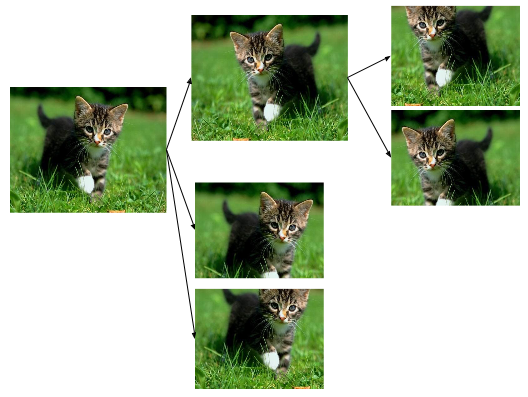
\includegraphics[scale=0.6,natwidth=528,natheight=397]{figures/dataAugmentationImage.png}
			\caption{Exemple d\textquotesingle augmentation de donn\'ee pour une image. Ici, on a obtenu six images \`a partie d\textquotesingle une seule. On a d\textquotesingle abord appliqu\'e une inversion d\textquotesingle image et puis on a rogn\'e les images obtenues de deux mani\`eres diff\'erentes. En r\'ealit\'e, beaucoup plus de transformations sont appliqu\'ees, permettant de multiplier la base de donn\'ees des images de beaucoup (1024 dans~\cite{howard2013some}).}
			\label{fig:dataAugmentationChat}
		\end{figure}

		Beaucoup de m\'ethode de data-augmentation le sont pour les images, la question \'etant de savoir si parmi ces m\'ethodes, on peut en r\'eutiliser ou non. Par exemple, on ne peut pas r\'ealiser une r\'eflection sur une s\'erie temporelle. Cependant, l’approche de Krizhevsky dans \cite{krizhevsky2012imagenet} pour les donn\'ees d’entra\^inement avec une ACP pourrait \^etre r\'ealisable sur des s\'eries temporelles. On pourrait peut-\^etre aussi rajouter du bruit contrôl\'e selon diff\'erents param\`etres comme dans \cite{krizhevsky2012imagenet} et \cite{howard2013some}.


\bigbreak
\bigbreak
\section{Conclusion}
Pour conclure , il existe de nombreuses mani\`eres d\textquotesingle augmenter le volume des donn\'ees. Cependant, ces m\'ethodes d\'ependent du type de donn\'ees. Avant de commencer \`a classifier des s\'eries temporelles, il va donc falloir trouver comment augmenter ce volume. Nous pourrions, par exemple, utiliser l\textquotesingle agorithme ACP ou s\textquotesingle inspirer des m\'ethodes utilis\'es sur les images.
Pour la classification, les CNN semblent \^etre un bon choix \'etant donn\'ee les bons r\'esultats obtenus dans \cite{zheng2014time}. Pour cela, nous allons utiliser le framework Caffe (voir \cite{jia2014caffe}). Une fois mis en place, nous pourrions alors observer les r\'esultats.

\section*{References}
	\nocite{*}
	\bibliographystyle{plain}
	\bibliography{biblio}



\end{document}
%%% Local Variables:
%%% mode: latex
%%% TeX-master: t
%%% End:
